\documentclass[a4paper]{article}

\usepackage[utf8]{inputenc}
\usepackage[T1]{fontenc}
\usepackage{textcomp}
\usepackage[swedish]{babel}
\usepackage{amsmath, amssymb}
\usepackage{physics}

% figure support
\usepackage{import}
\usepackage{xifthen}
\pdfminorversion=7
\usepackage{pdfpages}
\usepackage{transparent}
\usepackage{float}
\usepackage{parskip}
\newcommand{\incfig}[1]{%
	\def\svgwidth{\columnwidth}
	\import{./figures/}{#1.pdf_tex}
}

\pdfsuppresswarningpagegroup=1

\title{Assignment 1}
\author{Johan Ribbing \thanks{Thanks to}}
\date{maj 2021}

\begin{document}

\begin{titlepage}
\maketitle
\end{titlepage}

\begin{figure}[h]
	\centering
	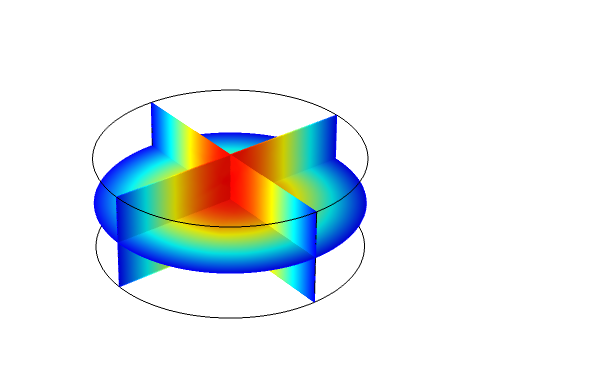
\includegraphics[width=0.8\textwidth]{3_52_normE.png}
	\caption{3.52 normE}
	\label{fig:352norme}
\end{figure}

\begin{figure}[h]
	\centering
	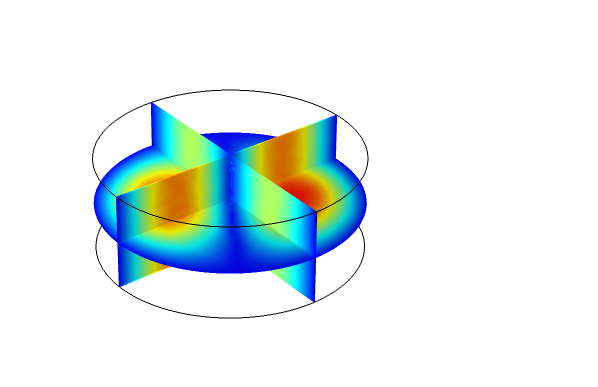
\includegraphics[width=0.8\textwidth]{5_61_normE.png}
	\caption{5.61 normE}
	\label{fig:561norme}
\end{figure}

\begin{figure}[h]
	\centering
	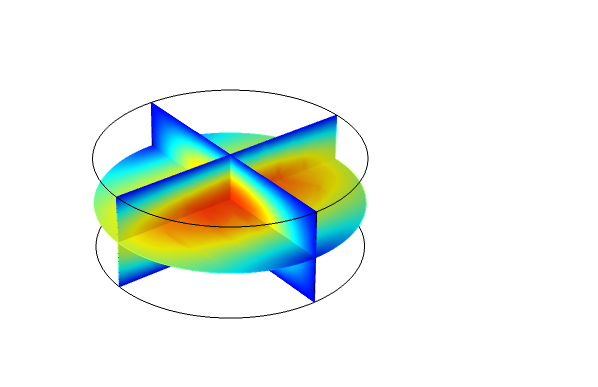
\includegraphics[width=0.8\textwidth]{6_66_normE.png}
	\caption{6.66 normE}
	\label{fig:666norme}
\end{figure}

\begin{figure}[h]
	\centering
	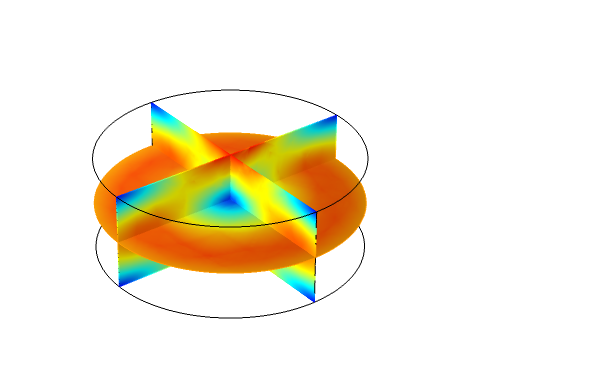
\includegraphics[width=0.8\textwidth]{7_04_normE.png}
	\caption{7.04 normE}
	\label{fig:704norme}
\end{figure}

\begin{figure}[h]
	\centering
	\includegraphics[width=0.8\textwidth]{bandstopbred_fält.png}
	\caption{dålig bandpass fältbild}
	\label{fig:bandpassfält}
\end{figure}

\begin{figure}[h]
	\centering
	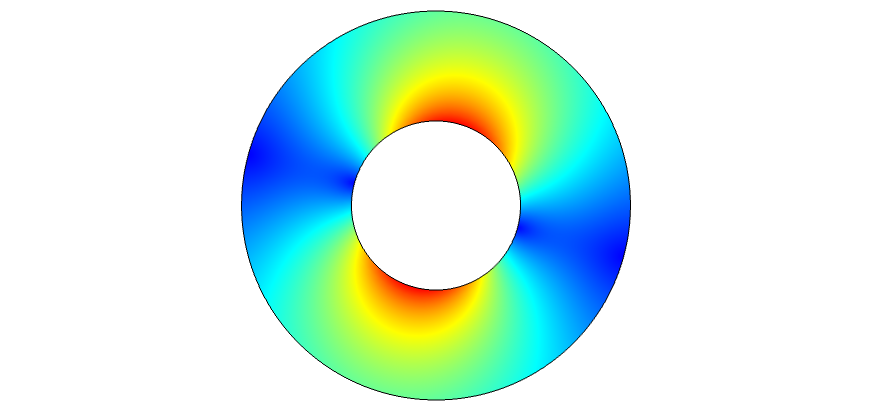
\includegraphics[width=0.8\textwidth]{coax_second_mode_normE.png}
	\caption{coax second mode normE}
	\label{fig:coaxnorme}
\end{figure}

\begin{figure}[h]
	\centering
	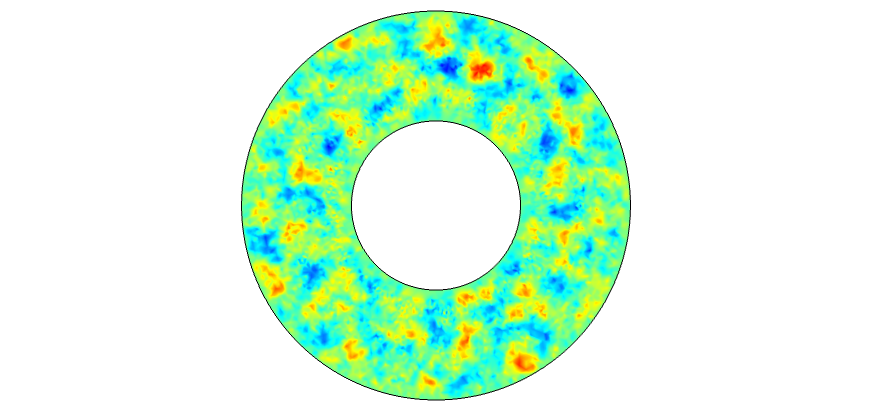
\includegraphics[width=0.8\textwidth]{coax_second_mode_Ez.png}
	\caption{coax second mode Ez}
	\label{fig:coaxez}
\end{figure}

\begin{figure}[h]
	\centering
	\includegraphics[width=0.8\textwidth]{fältbild_stark.png}
	\caption{fältbild stark}
	\label{fig:stark}
\end{figure}

\begin{figure}[h]
	\centering
	\includegraphics[width=0.8\textwidth]{fältbild_svag.png}
	\caption{fältbild svag}
	\label{fig:svag}
\end{figure}

\begin{figure}[h]
	\centering
	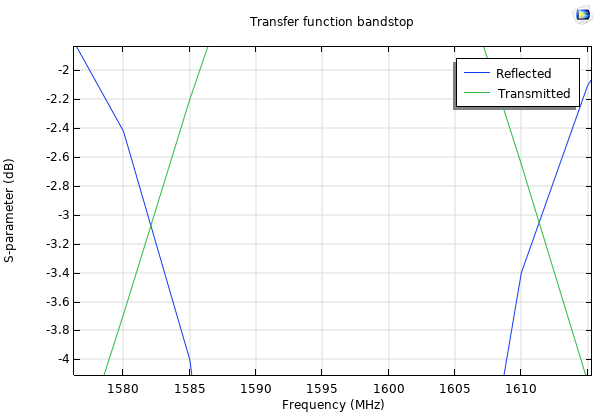
\includegraphics[width=0.8\textwidth]{reflect_transmit_dB_zoom.png}
	\caption{S param dB zoom}
	\label{fig:rtzoom}
\end{figure}

\begin{figure}[h]
	\centering
	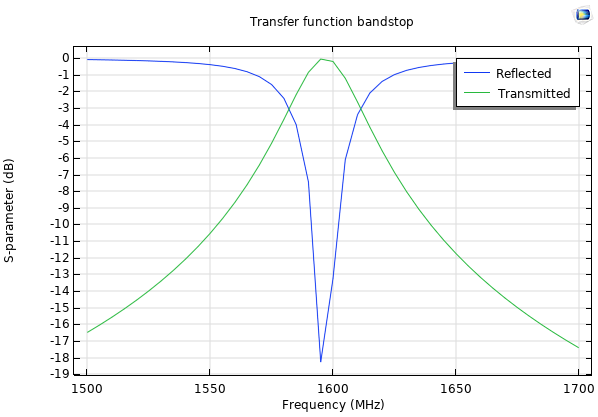
\includegraphics[width=0.8\textwidth]{reflect_transmit_dB.png}
	\caption{S param dB}
	\label{fig:rt}
\end{figure}

\begin{figure}[h]
	\centering
	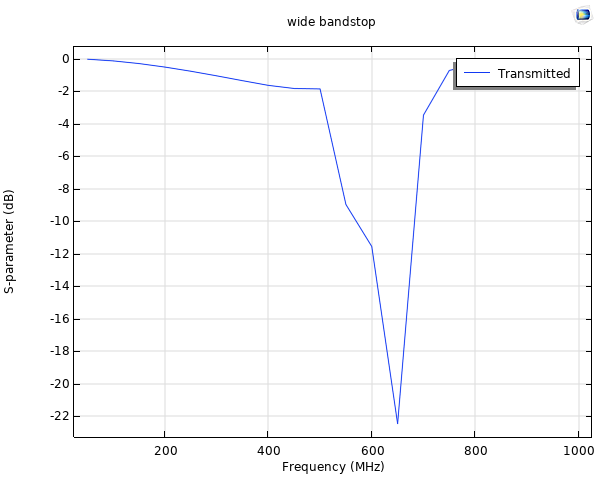
\includegraphics[width=0.8\textwidth]{bandstopbred.png}
	\caption{Transmission dålig bandpass}
	\label{fig:bandpass}
\end{figure}
	
\end{document}
